\item O pinhão $A$ roda sobre as cremalheiras $B$ e $C$. Se $B$ está se deslocando para a direita a \SI{2.4}{\meter/\second} e $C$ está se deslocando para a esquerda a \SI{1.2}{\meter/\second}, determine a velocidade angular do pinhão e a velocidade de seu centro $A$.

\import{../answers/}{answer-6}

\vspace{-1.5cm}
\begin{flushright}
	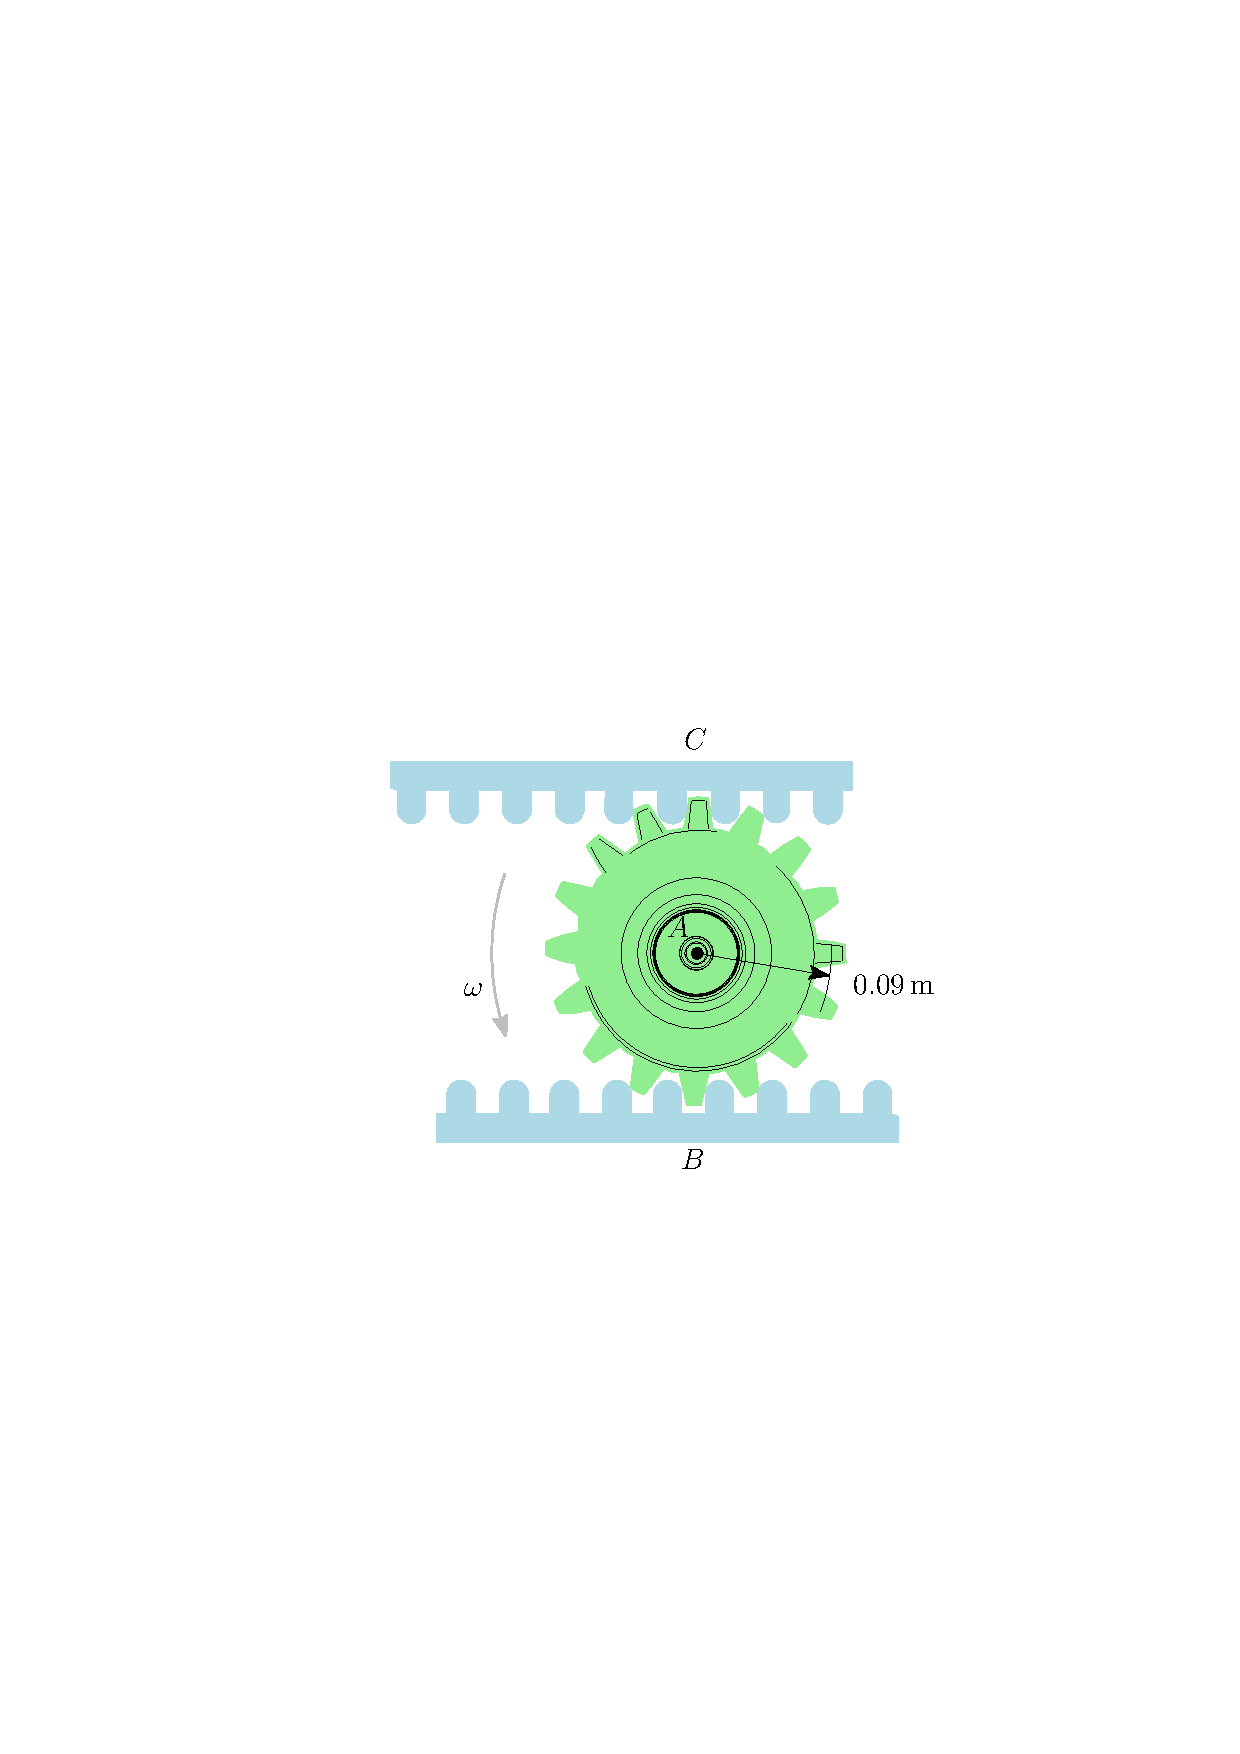
\includegraphics[scale=.95]{images/draw_4}
\end{flushright}